\documentclass[12pt]{article}

\usepackage[utf8]{inputenc}
\usepackage[english, russian]{babel}

\usepackage{slides}

% ШРИФТЫ
% Нужны рубленные шрифты -- раскомментируйте стоку ниже. 
% Нужны шрифты с засечками --- закомментируйте эту строку. 
\renewcommand{\familydefault}{\sfdefault} % Переключает на рубленный шрифт.
% Шрифты Times и Arial, если стоит пакет cyrtimes. 
% Если он не стоит, результат будет плохой!
%\usepackage{cyrtimespatched}
% Если нет cyrtimes, то попробуйте включить полужирный шрифт:
% \renewcommand{\seriesdefault}{b} % для шрифта с засечками, это предпочтительно
% \renewcommand{\seriesdefault}{sbc} % для рубленного шрифта

\usepackage{graphicx}
\usepackage{alltt}

\def\Student{Коротков Иван Андреевич}
\def\Advisor{Крищенко Всеволод Александрович}
\def\Title{Параллельное построение пространства состояний конечной модели}
\def\SubTitle{Квалификационная работа магистра}

% Верхний заголовок: пустой
% Нижний заголовок по-умолчанию:
% \lfoot{\Title} % слева
% \cfoot{} % цент пуст
% \rfoot{\thepage} % справа

% \renewcommand{\baselinestretch}{1.5}
 \linespread{1.2}

\hyphenpenalty=0

\begin{document}

\TitleSlide

\section{Цель}
\label{sec:goal}

\mbox{}

\mbox{}

\hline
\begin{center}
  Разработка и исследование метода параллельной генерации состояний конечной модели.
\end{center}
\hline

\section{Задачи}
\label{sec:tasks}

\small
\begin{itemize}
\item Определение применимости существующих методов построения пространства состояний для
  параллельных вычислений.
\item Выбор распределения состояний по узлам вычисления.
\item Проектирование и реализация алгоритма параллельного построения пространства состояний.
\item Трансляция формального описания системы в программный код для генерации состояний.
\item Тестирование реализованного алгоритма и проведение экспериментов.
\item Интерпретация результатов.
\end{itemize}
\normalsize

% \section{Ошибки в ПО}
% \label{sec:sw-errors}

% \begin{tabular}[ht]{|p{0.3\textwidth}|p{0.3\textwidth}|p{0.3\textwidth}|}
%   \hline 
%   Вероятность возникновения & Критические & Некритичные \\
%   \hline
%   высокая & Тестирование, верификация & Тестирование \\
%   \hline
%   низкая & Верификация & \\
%   \hline
% \end{tabular}

% \textit{Старый слайд, удалить?}

\section{Проблемы верификации конечных моделей}
\label{sec:verif-troubles}

\begin{itemize}
\item Размер пространства состояний растет экспоненциально

\item Модели среднего размера требуют более 10 Гб оперативной памяти для хранения пространства состояний

\item На верификацию средней модели уходят недели
\end{itemize}

\section{Уменьшение затрат на хранение состояний}
\label{sec:ram-lightening}

Генерация состояний:

\begin{itemize}
\item Последовательная
  \begin{itemize}
  \item Битовое хэширование
  \item Сжатие состояний
  \item Сокращение частных порядков
  \end{itemize}
\item Параллельная
\end{itemize}

\section{Работы в области параллельной генерации состояний}
\label{sec:analogues}

\begin{itemize}
\item Flavio Lerda, Riccardo Sisto. Distributed-Memory Model Checking with SPIN. Lecture
  Notes In Computer Science, vol. 1680, pp 22-39.

\item Jiri Barnat, Lubos Brim. Parallel Breadth-First Search LTL Model-Checking. 18th IEEE
  International Conference on Automated Software Engineering (ASE'03), pp. 106-115.
\end{itemize}

\section{Распределение ролей между узлами}
\label{sec:par-gen}

\begin{itemize}
\item Распределенное хранилище состояний
  \begin{itemize}
  \item Генерация состояний только на одном узле
  \item Неэффективно из-за неиспользования вычислительных ресурсов и большого количества
    удаленных вызовов
  \item Позволяет выполнять обход в глубину и поиск циклов
  \end{itemize}

\item Распределенная генерация состояний
  \begin{itemize}
  \item Каждый узел является хранилищем и генератором
  \item Используются вычислительные ресурсы всех узлов
  \item Необходимо использовать поиск в ширину: поиск циклов затруднен
  \end{itemize}

\end{itemize}

\section{Псевдокод метода \\ <<Распределенная генерация состояний>>}
\label{sec:par-pseudocode}

\scriptsize
\begin{verbatim}
Visited = []
Queue = []

if NodeId = 0:
    Queue += start_state

while not empty(Queue):
    state <- Queue
    node = StateNode(state)
    if NodeId = node:
        if not state in Visited:
            Visited += state
            for each state' in Next(state):
                Queue <- state'
    else:
        node.Queue <- state
\end{verbatim}
\normalsize

\section{Распределение состояний между узлами}
\label{sec:state-partitioning}

\begin{center}
  \includegraphics[width=0.9\textwidth]{../graphics/state-partition}
\end{center}

\section{Сравнение распределений на основе полученных результатов}
\label{sec:partition-compare}

\begin{tabular}[ht]{|r|l|l|p{0.25\textwidth}|p{0.25\textwidth}|}
  \hline 
  P & Состояния & Переходы & Удаленные вызовы & Загруженность узлов    \\ \hline
  5 & 28351     & 42658    & 31356  (73\%)/ 7047  (16\%) & 0.99 / 0.66 \\ \hline
  6 & 147774    & 232748   & 170378 (73\%)/ 31668 (13\%) & 0.99 / 0.68 \\ \hline
  7 & 360354    & 601462   & 453789 (75\%)/ 66438 (11\%) & 0.99 / 0.74 \\ \hline
\end{tabular}

\section{Взаимодействие узлов (MPI)}
\label{sec:mpi-interaction}

\begin{center}
  \includegraphics[height=0.8\textheight]{../graphics/mpi-async-seq}
\end{center}

\section{Хранение состояний \\ \small{Полное хэширование}}
\label{sec:fullstate}

\begin{center}
  \includegraphics[height=0.8\textheight]{../graphics/fullstate}
\end{center}

\section{Хранение состояний \\ \small{Битовое хэширование}}
\label{sec:buthash}

\begin{center}
  \includegraphics[height=0.7\textheight]{../graphics/bitstate}
\end{center}

\section{Распределенное завершение}
\label{sec:distributed-termination}

\begin{center}
  \includegraphics[width=1\textwidth]{../graphics/distr-termination}
\end{center}

\section{Нотация PROMELA}
\label{sec:promela-notation}

%              <--------------------- глобальные переменные 
%     <------ класс процесса (3 начальных экземпляра)

\begin{minipage}[t]{.53\textwidth}
\scriptsize
\begin{verbatim}
byte fork[3]
byte nr_eat

active [3] proctype Philosopher() { 
Think:
  atomic { fork[_pid] == 0 -> 
           fork[_pid] = 1 };
One:
  atomic { fork[(_pid + 1)%3] == 0 -> 
           fork[(_pid + 1)%3] = 1; nr_eat++ };
Eat:
  atomic { nr_eat--; fork[(_pid + 1)%3] = 0 };
  fork[_pid] = 0;
  goto Think
}
\end{verbatim}
\normalsize
\end{minipage}
%
\begin{minipage}[t]{.47\textwidth}
\scriptsize
\begin{verbatim}
Глобальные переменные


класс процесса (3 начальных экземпляра)

условие выполнимости
действие

внутри atomic может быть лишь один процесс




бесконечный цикл в каждом процессе

\end{verbatim}
\normalsize
\end{minipage}

% \begin{minipage}[m]{.34\textwidth}
% \centerline{Результаты}
% \end{minipage}
% %
% \begin{minipage}[m]{.65\textwidth}

% Для вёрстки отдельных слайдов в две колонки используется окружение
%   \verb+minipage+.

% Пример кода с неравномерными колонками (для равномерных используйте 49 и 49):

% \begin{verbatim}
% \begin{minipage}[m]{.34\textwidth}
%   \includegraphics...
% \end{minipage}
% \begin{minipage}[m]{.64\textwidth}
%   Текст
% \end{minipage}
% \end{verbatim}

% Недостаток использования \verb+minipage+ --- исчезают интервалы между абзацами.
% \end{minipage}

\section{Процесс верификации конечной модели}
\label{sec:idef0}

\begin{center}
  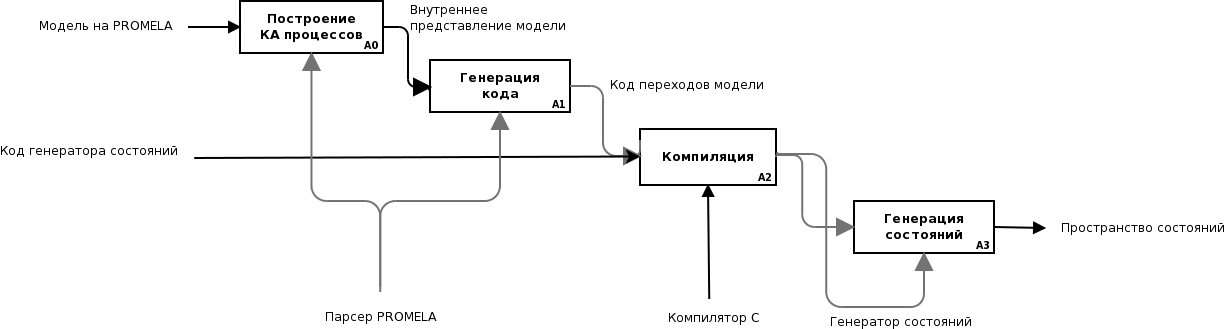
\includegraphics[width=1.0\textwidth]{../graphics/idef0-codegen}
\end{center}

\section{Представление состояний}
\label{sec:state-represent}

\begin{center}
  \includegraphics[height=0.8\textheight]{../graphics/state-representation}
\end{center}

\section{Публикации}
\label{sec:publications}

По результатам работы имеется одна публикация:

И.\,Коротков. Параллельное построение пространства состояний конечной системы. Новые
информационные технологии в автоматизированных системах: материалы тринадцатого
научно-практического семинара.~-- Моск. гос. ин-т электроники и математики. М., 2010,
стр.~169-176.

\section{Итоги}
\label{sec:publications}

\small
\begin{itemize}
\item Найдено распределение состояний между узлами, значительно сокращающее накладные
  расходы на удаленные вызовы;
\item спроектировано и реализовано параллельное построение пространства состояний;
\item реализованы 2 различных схемы хранения состояни;
\item реализован транслятор для нотации PROMELA;
\end{itemize}
\normalsize

\end{document}
